\documentclass{article}

\newif\ifBenchTikzExternalize
\BenchTikzExternalizefalse
\newif\ifBenchMintedCache
\BenchMintedCachefalse
\InputIfFileExists{bench-config.tex}{}{}

\newcommand{\benchtexttoken}{ALPHA}
\newcommand{\benchfiguretoken}{1.00}
\newcommand{\benchpreambletoken}{P0}

\usepackage{fontspec}
\usepackage{hyperref}
\usepackage{tikz}

\setmainfont{TeX Gyre Pagella}
\setsansfont{TeX Gyre Heros}[Scale=MatchLowercase]
\setmonofont{TeX Gyre Cursor}[Scale=MatchLowercase]
\hypersetup{pdfsubject={FastXeBench fontspec validation \benchpreambletoken}}

\title{R1 Fontspec Example Validation}
\author{Derived from the local fontspec package example}
\date{}

\begin{document}
\maketitle
\pagestyle{empty}

\section*{The basics of the \textsf{fontspec} package}

This real-project-derived workload preserves the original font selection example while adding a controlled edit token \benchtexttoken{} and an active citation path \cite{refalpha}.

The \textsf{fontspec} package enables automatic font selection
for \LaTeX{} documents typeset with Xe\TeX{} or Lua\TeX.
The basic command is

{\centering \verb|\fontspec{font display name}[font features]|.\par}

The default, sans serif, and typewriter fonts may be set with the
commands \verb|\setmainfont|, \verb|\setsansfont| and \verb|\setmonofont|,
respectively, as shown in the preamble. They take the
same syntax as the \verb|\fontspec| package. All expected font
shapes are available:

\begin{center}
  {\itshape Italics and \scshape small caps\dots}\\
  {\sffamily\bfseries Bold sans serif and \itshape bold italic sans serif\dots}
\end{center}

Text fonts in maths mode are also changed (e.g., notice the cosine function in
`$\cos(n\pi)=\pm 1$') but only if the roman and sans serif fonts are set in
the preamble; \verb|\setmainfont| will not affect these maths mode fonts when
called mid-document.
Maths symbols themselves are not affected.

Notice the font features used to load the default fonts in the preamble.
\verb|Ligatures=TeX| is automatically enabled for the roman and sans font,
allowing regular \TeX{} ligatures like \verb|``---''| for ``---''.
\verb|Scale=MatchLowercase| automatically scales the fonts to
the same x-height.

\begin{figure}[h]
\centering
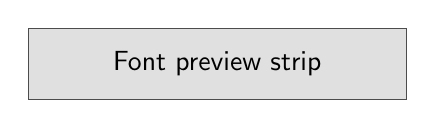
\begin{tikzpicture}[scale=\benchfiguretoken]
  \draw[fill=black!12, draw=black!70] (0,0) rectangle (4.8,0.9);
  \node at (2.4,0.45) {\sffamily Font preview strip};
\end{tikzpicture}
\caption{A small figure surrogate added for the figure-edit scenario.}
\label{fig:fontspec-strip}
\end{figure}

Please see the complete \textsf{fontspec} documentation for further
information; Figure~\ref{fig:fontspec-strip} keeps a simple graphics path active for validation purposes.

\bibliographystyle{plain}
\bibliography{refs}

\end{document}
